%%% Time-stamp: <2016-04-18 01:32:05, v1.3 sunthar>
%%% $Log:$
% This document describes how to use iitbreport style
%********************************************************************

%\documentclass[11pt,a4paper,openright]{report}
\documentclass[twoside]{iitbreport}

%% Default spacing: 1.5
%% Default font size: 12pt
%% Default font: txfonts (similar to times new roman) 

%% Selectively comment out sections that you want to be left out but
%% maintaining the page numbers and other \ref
\includeonly{%
  intro/introduction,
  lit/literature,
  expt/experimental,
  rnd/results, 
  dec,abs,pub,ack
}

%%% Some commonly used packages (make sure your LaTeX installation
%%% contains these packages, if not ask your senior to help installing
%%% the packages)

\usepackage{booktabs}
\graphicspath{{expt/}}


%%% Macro definitions for Commonly used symbols
\newcommand{\Rey}{\ensuremath{\mathrm{Re}}}
\newcommand{\avg}[1]{\ensuremath{\overline{#1}}}
\newcommand{\tenpow}[1]{\ensuremath{\times 10^{#1}}}
\newcommand{\pder}[2]{\ensuremath{\frac{\partial#1}{\partial#2}}}

% Referencing macros
\newcommand{\Eqref}[1]{Equation~\eqref{#1}}
\newcommand{\Tabref}[1]{Table~\ref{#1}}
\newcommand{\Figref}[1]{Figure~\ref{#1}}
\newcommand{\Appref}[1]{Appendix~\ref{#1}}


\begin{document}
	
%%********************************Frontmatter***********************
% In frontmatter everything comes with roman numbering	
\pagenumbering{roman}
\setcounter{page}{1}

%*******************************************************************
%                         Title Page                            
%*******************************************************************
\title{Essential \LaTeX\ Templates for Report Writing}
\author{My name}

%% Print the date. Today's date comes by default, change it here to 
%% other date format, if required:

%\date{\today}
%\date{10 Mar 2016}


%% The type of the report can be set here

\reporttype{A Seminar Report}
%\reporttype{A Thesis}
%\reporttype{A Dissertation}
%\reporttype{A Project Report}

%% Name of the degree
\degree{Doctor of Philosophy}
%\degree{Master of Technology}


%% Department/Centre Name
\dept{Department of Chemical Engineering}

%% Supervisor and cosupervisor/excosupervisor name can be put here
\supervisor{Supervisor name}
%\cosupervisor{Unknown name}
%\excosupervisor{Unknown name}

%% Roll number
\rollnum{Roll No. ....}

\maketitle

%*******************************************************************
%                         Copyright Page                          
%******************************************************************* 
%\mycopyright                    

%*******************************************************************
%                         Dedication Page                         
%*******************************************************************
\dedication[Dedicated to \ldots]        
%\addintoc{Dedication}

%*******************************************************************
%                        Certificate Page                         
%*******************************************************************
%\makecertificate[change title name]{report type} 
\makecertificate{seminar report} 
%\makecertificate{thesis}
%\makecertificate{dissertation}
%\makecertificate{project report}

%\addintoc{Certificate}

%*******************************************************************
%                         Approval Sheet                         
%*******************************************************************
%\makeapproval{thesis}
%\makeapproval{dissertation}

%*******************************************************************
%                          Declaration                           
%*******************************************************************
%==================================dec.tex================================
%
\begin{Declaration}
\noindent
I declare that this written submission represents my ideas in my own words and where others' ideas or words have been included, I have adequately cited and referenced the original sources. I declare that I have properly and accurately acknowledged all sources used in the production of this report. I also declare that I have adhered to all principles of academic honesty and integrity and have not misrepresented or fabricated or falsified any idea/data/fact/source in my submission. I understand that any violation of the above will be a cause for disciplinary action by the Institute and can also evoke penal action from the sources which have thus not been properly cited or from whom proper permission has not been taken when needed.

%
%
%
%
%
%
%

\DecSign[\today]



%
\end{Declaration}
%========================================================================
















 
%\addintoc{Declaration}

%******************************************************************
%                          Abstract                             
%******************************************************************  
%============================= abs.tex================================
\begin{Abstract}
This document contains essential templates required to write technical
reports using \LaTeX.  Particularly it shows how to create an
equation, figure, table, symbols list, and bibliographic citation in a \LaTeX\
document.
%
%
%
%
%
\end{Abstract}
%=======================================================================

                    

%******************************************************************
%                         Contents list                         
%******************************************************************
%\figurespagefalse
%\tablespagefalse
\makecontents % Creats toc, lof, and lot

%******************************************************************
%                        Notations                              
%******************************************************************
\notations[4cm]{List of Symbols}      

%%********************************Mainmatter***********************
% In mainmatter everything comes with arabic numbering	
\cleardoublepage
\setcounter{page}{1}
\pagenumbering{arabic}

%******************************************************************
%                         Chapters                           
%****************************************************************** 

\newcommand{\etas}{\ensuremath{\eta_{\mathrm{s}}}}


\chapter{Introduction}


This document contains commonly used essential templates to write a
\LaTeX\ document. This document is to be used along with the files and
folders provided. Writing a \LaTeX\ document is very simple.  Often
students need only very simple constructs.  This document shows
certain essential features that almost all technical report writing
requires. Please consult the PDF file for the output of the document,
and then look at the corresponding \LaTeX\ file to reproduce it.  The
document illustrates the following constructs
\begin{itemize}
\item Unnumbered and numbered Lists
\item Equations
\item Defining short macros for frequently used symbols
\item Bibliography
\item Figures
\item Tables
\end{itemize}

The normal procedure for compiling a \LaTeX\ document that contains
bibliographic entries is to follow the following steps
\begin{enumerate}
\item \verb|pdflatex mainrep|
\item \verb|bibtex mainrep|
\item \verb|pdflatex mainrep|
\item \verb|pdflatex mainrep|
\end{enumerate}
In the above example \verb|mainrep| is the main \LaTeX\ file.


\section{First section of this chapter}

This is the first chapter, which resides in a directory (folder)
intro. Each chapter can contain \verb|section|, \verb|subsection|
and so on.

\subsection{Equations and Math symbols}


Equations should be set in a separate mode.  For details on getting
various types of aligned equations, consult the \AmS-\LaTeX\
documentation \verb|amsldoc.pdf|. Simple equations are set as
\begin{equation}
\label{eq:sinx}
\int \mathrm{d}x \; \cos x =  \sin x
\end{equation}
Equation~\eqref{eq:sinx} is the integral of the cosine
function. Mathematical symbols must always be put inside \verb|$$|,
when they appear outside a math environment (such as \verb|equation|,
\verb|align|, \verb|gather|, etc).  The symbol ``ex'' must be written as
$x$ and not as x.  

Another commonly used construct for equations is the \verb|align|
environment to align several equations along a vertical line. It is
usually the $=$ sign across which the alignment is done.  The
point of alignment for each equation is specified using the ampersand symbol 
\begin{align}
a &= b  \\
a + e + f + g & = m + n + z \\
x + 2 & = x^{3} + 3 x^{2} + 2 x + 5
\end{align}

\subsection{Commonly used Symbols}
For mathematical symbols it is very convenient to define frequently
used symbols as a short macro. For example if you are to be using the
symbol $\eta_{\mathrm{s}}$ frequently it is convenient to define it in
as:\\
\verb|\newcommand{\etas}{\ensuremath{\eta_{\mathrm{s}}}}| \\
in the preamble and to simply refer it to in the text as \etas\ or in
a mathematical equation as $\etas = \eta \, ( 1 + \phi)$.
%%
%

\section{How to write nomenclature} 

\subsection{General guidelines:}
\begin{enumerate}	
	\item Use \verb|\nomenclature[prefix]{symbol}{description}| for symbols, the best place for this command is immediately after you introduce the symbol for the first time
	\item Shorten the long command:\\ \verb|\newcommand{\nm}[2]{\nomenclature{#1}{#2}}|
	\item Create compiler for nomenclature with the given code: \\
	\textbf{makeindex \%.nlo -s nomencl.ist -o \%.nls -t \%.nlg }\\
	For TeXstudio: go to options > build > user command > write- `user1: Nomenclature' amd paste the above code\\
	For compiling the nomenclature: go to tools > user > Nomenclature	
\end{enumerate}	

\subsection{Grouped nomenclature}
\begin{enumerate}
\item For acronyms, use:\\
 \verb|\nmA[sorting letter]{symbol}{descritpon}|
\item For roman symbols, use:\\
\verb|\nmR[sorting letter]{symbol}{descritpon}|
\item For greek symbols, use:\\
 \verb|\nmG[sorting letter]{symbol}{descritpon}|
 \item For superscripts, use:\\
 \verb|\nmS[sorting letter]{symbol}{descritpon}|
 \item For subscripts, use:\\
 \verb|\nms[sorting letter]{symbol}{descritpon}| 
 \item For any other symbol, use:\\
 \verb|\nmX[sorting letter]{symbol}{descritpon}|\\
 Name of other symbols can be changed with \verb|\OtherSym{Name of symbols}|
\end{enumerate}
%%
\subsection{Some examples}
\begin{enumerate}
\item \verb|\nmA[FF]{FFA}{Free fatty acid}|
\item \verb|\nmA[AO]{AOR}{Angle of repose}|
\item \verb|\nmR[Ra]{$R$}{Radius of circle}|
\item \verb|\nmR[ra]{$r$}{Intrinsic length}|
\item \verb|\nmR[Gr]{$G_\mathrm{r}$}{Gravity}|
\item \verb|\nmG[al]{$\alpha_{\mathrm{a}}$}{Angular acceleration}|
\item \verb|\nmG[et]{$\eta$}{Viscosity}|
\item \verb|\nmG[be]{$\beta$}{Shape factor}|
\item \verb|\nmS[v]{$v$}{Vapor phase}|
\item \verb|\nmS[g]{$g$}{Gas phase}|
\item \verb|\nms[i]{$i$}{Indices}|
\item \verb|\nms[x]{$x$}{Variable in x-direction}|
\item \verb|\nmX[f]{foo}{foo|
\end{enumerate} 

\nmA[FF]{FFA}{Free fatty acid}
\nmA[AO]{AOR}{Angle of repose}


\nmR[Ra]{$R$}{Radius of circle}
\nmR[ra]{$r$}{Intrinsic length}
%\nmR[Gr]{$G_\mathrm{r}$}{Gravity}


\nmG[al]{$\alpha_{\mathrm{a}}$}{Angular acceleration}
\nmG[et]{$\eta$}{Viscosity}
%\nmG[be]{$\beta$}{Shape factor}


\nmS[v]{$v$}{Vapor phase}
\nmS[g]{$g$}{Gas phase}


\nms[i]{$i$}{Indices}
\nms[x]{$x$}{Variable in x-direction}


\nmX[f]{foo}{foo}


%%


%%% Local Variables: 
%%% mode: latex
%%% TeX-master: "../mainrep"
%%% End: 


\chapter{Literature Survey}

The bibliographic entries are to be kept in a file named
\verb|<something>.bib|. In this sample report we call it as
\verb|mylit.bib|. This file must be included without the \verb|.bib|
extension in the main file as: \verb|\bibliography{mylit}|.   Open the
file \verb|mylit.bib| to see the format in which the entries are
written. This is written in the Bib\TeX format. Most of the
bibliographic web pages (Scopus, ISI Web) and software (EndNote, etc)
allow you to export bibliographic entries in the Bib\TeX format.

Citations are referred in the text using \verb|\citet| command which produces
citations as though they are part of the text.  In order to say
somebody did this work as a part of a line use: \verb|\citet{Auth09}|
have done extensive work on \ldots.  This will produce

\citet{Auth09} have done extensive work on \ldots


Alternately citations can appear in parenthesis.  The
command \verb|\citep{Auth09}| is used to automatically put the
citations in parenthesis.
  As an example consider the extensive work
done in the area of book writing \citep{Mono08,Auth09}.

%%% Local Variables: 
%%% mode: latex
%%% TeX-master: "../mainrep"
%%% End: 


\chapter{Materials and Methods}

\section{Including Figures}

Figures are conveniently included using postscript format.  If you are
generating a figure in a software, please check if the software
supports writing to a postscript or a PDF format. This format is loss
less vector format and with reproduce in any magnification without any
pixelation. Make sure to write it to an ``Encapsulated Post-script''or
.eps format.


\begin{figure}[tbp]
  \centering
    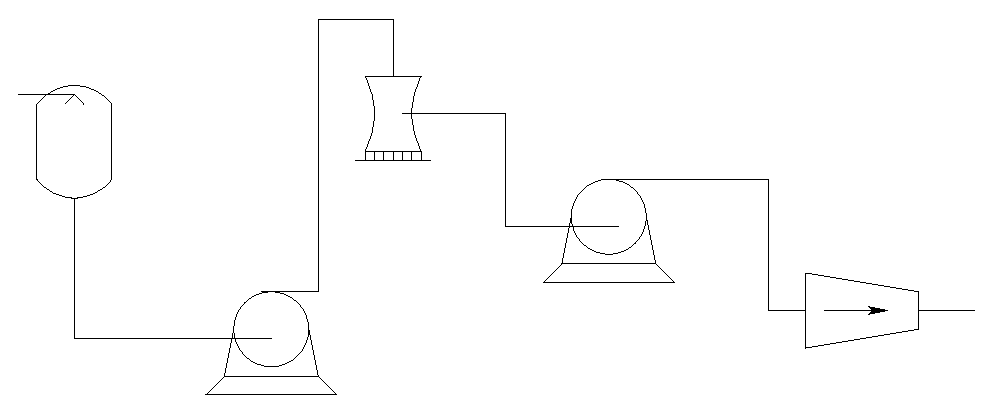
\includegraphics[width=0.7\textwidth]{profflow}
    \caption[Process flow sheet]{Process flow sheet of the
      experimental setup. The caption of the figure goes here. A
      shorter caption can be written in square brackets to identify it
      in the list of figures.}
    \label{fig:pfs} 
\end{figure}

Figures should be given a label and which can be used to refer to them
in the running text using \verb|\ref{}| command. Figure~\ref{fig:pfs}
describes the process flow sheet of the experimental set up used in
this report. The \Figref{fig:pfs} can also be refered by a short form notation
a pre-defined macro \verb"\Figref".



%%% Local Variables: 
%%% mode: latex
%%% TeX-master: "../mainrep"
%%% End: 

\chapter{Results and Discussions}


\section{Including Tables}

Tables are to be used in a special environment so that they have a
Number, caption and appear in the list of tables.
Table~\ref{tab:samtab} is a sample table. In the case of tables, it is
a convention to write the caption above the table.  Note that in the
case of figures the caption appears below the figure.

\begin{table}[tbp]
  \centering
    \caption{Physical properties of the materials used.}
    \label{tab:samtab}
    \begin{tabular}{ll}
      \toprule 
      Property & Value \\
      \midrule
      Particle Density, $\rho_{\mathrm{p}}$ & 2500 kg/m$^{3}$ \\
      Viscosity, $\eta_{\mathrm{s}}$& 1 $\times 10^{-3}$ Pa-s \\
      \bottomrule \\
    \end{tabular}  
\end{table}

%%% Local Variables: 
%%% mode: latex
%%% TeX-master: "../mainrep"
%%% End: 


%****************************************************************
%                         Appendices                           
%****************************************************************
%% Additional, supporting material, such as codes, derivations, etc., can be placed in the appendix
\appendix
\chapter{Supporting Material}

%******************************************************************
%                         Bibliography or References          
%******************************************************************  
\bibliography{mylit}     

%*******************************************************************
%                         List of publications               
%******************************************************************
%%%
\listofpublications


\noindent Put your publications from the thesis here. The packages \texttt{multibib} or \texttt{bibtopic} or \texttt{biblatex} or enumerate environment or thebibliography environment etc. can be used to handle multiple different bibliographies in the document.








%%======================================================================
%%% Local Variables: 
%%% mode: latex
%%% TeX-master: "../mainrep"
%%% End: 







            

%*******************************************************************
%                        Acknowledgements                    
%******************************************************************* 
%%%
\acknowledgments

This section is for the acknowledgments. Please keep this brief and resist the temptation of writing flowery prose! Do include all those who helped you, e.g. other faculty/staff you consulted, colleagues who assisted etc.






\signature{\today}
%\signature[Indian Institute of Technology Bombay]{\today}

%========================================================================

%%% Local Variables: 
%%% mode: latex
%%% TeX-master: "../mainrep"
%%% End:            

%*******************************************************************
%                        About author                    
%*******************************************************************
\colophon % remove this command while using this file.

% GAME OVER
%*******************************************************************
\end{document}

%%% Local Variables: 
%%% mode: latex
%%% TeX-master: t
%%% End: 
